\chapter[Our Framework at Work on the iTrust SWaT System]{Our Framework at Work: Reverse Engineering of the iTrust SWaT System}
\label{application}
\linenumbers

\lettrine{I}{n this} chapter, our main objective is to apply the framework and methodology introduced in Chapter \ref{chap:proposal} to the case study of the iTrust SWaT system, as illustrated in Chapter \ref{casestudy}. The purpose of this analysis is to assess the effectiveness and potential of the proposed framework within the context of a system that closely replicates a real-world water treatment plant, albeit on a smaller scale.

\bigskip
Due to the complexity of the system and the limited space available in this thesis, we will not conduct a comprehensive analysis and reverse engineering of the entire system. Instead, we will focus on specific parts for analysis. We leave it to the reader or those interested in utilizing the proposed methodology and framework to complete the analysis, should they choose to do so.\newline
By focusing on selective components and leaving room for further exploration, we strike a balance between providing valuable insights and acknowledging the potential for additional research. This approach empowers the reader and interested individuals to explore the iTrust SWaT system further and leverage the proposed methodology and framework for a more comprehensive analysis.

\section{Preliminary Operations}
\label{sec:6_preliminar_operations}
Prior to beginning the actual analysis, several preliminary manual operations need to be conducted on the physical process dataset utilized as a case study, specifically the SWaT system dataset for the year 2015 as outlined in Section \ref{subsec:5_2015_datasets}. To simulate the data-capture process performed by Ceccato et al. using their scanning tool, the original dataset in XLSX format (proprietary to Microsoft Excel) was divided into multiple datasets in CSV format. Each of these datasets corresponds to the individual stages of the SWaT system and contains the respective registers. These resulting files were then saved in the directory specified by the \texttt{raw\_dataset\_directory} directive in the framework configuration file, \textit{config.ini}, ready to be used in the pre-processing phase.\newline
Furthermore, the headers were manually renamed by adding a prefix from \texttt{P1\_} to \texttt{P6\_} to each register's name. This prefix indicates the stages, ensuring that each register is easily identifiable and linked to its corresponding stage.

\section{Determining the Analysis Strategy}
\label{sec:6_analysis_strategy}
The complexity of the system being analyzed necessitates the adoption of a deliberate strategy for the analysis. It is not feasible to rely on trial and error or attempt every possible combination between stages. The former approach may overlook crucial relationships between PLCs or between registers, while the latter may result in excessive and unproductive efforts if the specific portion of the system being analyzed lacks significant information or relationships. \newline
A sound analysis strategy helps us focus on the important parts of the system, improving the quality of the analysis and leading to better process comprehension. By prioritizing our attention, we can gain a deeper understanding of the crucial components, resulting in more informed decision-making and a comprehensive understanding of the overall processes.

\bigskip
To define this strategy, a potential starting point could involve analyzing network traffic to determine the communication patterns and participants within the system. This can be accomplished by utilizing the techniques discussed in Section \ref{subsec:4_network_analysis} on Network Analysis. By applying the Python script described in that section to the data extracted from the network traffic dataset debated in Section \ref{par:5_2015_net_dataset}, we can generate a (simplified) network graph, as illustrated in Figure \ref{fig:6_network_SWaT}.

\begin{figure}[ht]
	\centering
	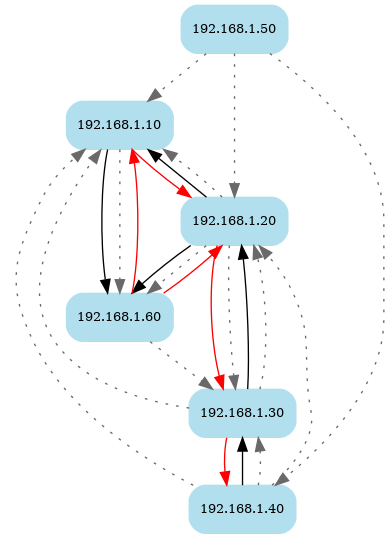
\includegraphics[scale=0.65]{chap6/network2.png}
	\caption{Simplified graph of the iTrust SWaT system network}
	\label{fig:6_network_SWaT}
\end{figure}

The graph clearly illustrates the structure of communications between the PLCs. Referring back to Table \ref{table:5_swat_ip_addresses}, which displays the IP address - PLC associations, we can observe that PLCs 1 through 4 communicate directly and sequentially with each other in a Request/Response communication pattern (represented by red and black arrows, respectively). Additionally, PLC6 communicates with both PLC1 and PLC2. On the other hand, the gray dotted arrows indicate communications for which we have knowledge of a response, but the corresponding request is unknown. For the purposes of our analysis strategy, we will not consider these communications within this context.

\bigskip
Based on our observations, the analysis strategy we will adopt involves considering sequential pairs of PLCs to effectively capture the relationships and implications between registers. Therefore, the PLC pairs we will focus on are PLC1-2, PLC2-3, and PLC3-4. This approach allows us to gain deeper insights into the interplay and dependencies between these PLC pairs.

\section{Reverse engineering of PLC1 and PLC2}
\label{sec:6_P1P2_analysis}

\subsection{Pre-processing}
\label{subsec:6_P1P2_preprocessing}

\subsection{Graphs and Statistical Analysis}
\label{subsec:6_P1P2_graphs}

\subsection{Invariant Inference and Analysis}
\label{subsec:6_P1P2_invariants}

\subsection{Business Process Analysis}
\label{subsec:6_P1P2_bpa}

\section{Reverse engineering of PLC2 and PLC3}
\label{sec:6_P2P3_analysis}

\subsection{Pre-processing}
\label{subsec:6_P2P3_preprocessing}

\subsection{Graphs and Statistical Analysis}
\label{subsec:6_P2P3_graphs}

\subsection{Invariant Inference and Analysis}
\label{subsec:6_P2P3_invariants}

\subsection{Business Process Analysis}
\label{subsec:6_P2P3_bpa}

\section{Reverse Engineering of PLC3 and PLC4}
\label{sec:6_P3P4_analysis}

\subsection{Pre-processing}
\label{subsec:6_P3P4_preprocessing}

\subsection{Graphs and Statistical Analysis}
\label{subsec:6_P3P4_graphs}

\subsection{Invariant Inference and Analysis}
\label{subsec:6_P3P4_invariants}

\subsection{Business Process Analysis}
\label{subsec:6_P3P4_bpa}

\vfill
\nolinenumbers